\documentclass[a4paper, 12pt]{article}
\usepackage[slovene]{babel}
\usepackage[utf8]{inputenc}
\usepackage[T1]{fontenc}
\usepackage{mathtools}
\usepackage{amsmath}
\usepackage{tikz}

\setlength{\parindent}{0px}
\setlength{\parskip}{10px}

\begin{document}

	\section*{Linearna regresija}
	\paragraph{}
	Predstavljajmo si, da izvajamo fizikalni poskus. Imamo vzmet, na kateri merimo raztezek v odvisnosti od sile, s katero napenjamo vzmet (na vzmet obešamo uteži z znano težo in merimo raztezek).

	\footnote{Podatki pridobljeni iz: \texttt{http://www.clemson.edu/ces/phoenix/labs/124/shm/}}
	\begin{tabular}{l|lllll}
		$F$ {[}N{]}  & 1  & 2  & 3  & 4  & 5  \\ \hline
		$x$ {[}cm{]} & 10 & 20 & 35 & 55 & 80
	\end{tabular}

	\paragraph{}
	Velja Hookov zakon, $F = k x$, torej sta $x$ in $F$ med seboj linearno odvisna. Poskušali bomo najti premico, ki se bo najbolje prilegala danim točkam v ravnini.

	\paragraph{}
	Če imamo 2 točki $T_1(x_1, y_1), T_2(x_2, y_2)$, lahko brez težav najdemo premico, ki gre točno skozi niju. Če pa je točk več, ni nujno, da obstaja premica, ki gre skozi vse točke.
	Iščemo taka $a$ in $b$, da se bo premica kar najbolje prilegala danim točkam. Če gre premica skozi neko točko $T_i(x_i, y_i)$, potem velja:

	$$0 = a x_i + b - y_i$$

	Ker pa naša premica ne poteka direktno skozi vse točke pride do napake, ki jo bomo v točki $T_i$ označili z $\varepsilon_i$.

	$$\varepsilon_i = a x_i + b - y_i$$

	\paragraph{}
	Napaka je lahko pozitivna ali negativna, odvisno ali točka leži pod ali nad premico. Želimo zmanjšati velikost vseh napak, ne glede na to, ali so pozitivne ali negativne. (Lahko bi preprosto sešteli absolutne vrednosti napak, ampak pozneje funkcije ne bi mogli odvajati.) Zato seštejemo kvadrate vseh napak.

	$$\varepsilon = \sum_{i=1}^{N} \varepsilon_i^2$$
	$$\varepsilon = \sum_{i=1}^{N} (a x_i - b - y_i)^2$$

	\paragraph{}
	Naš cilj je, da minimiziramo to napako. Minimum funkcije pa najdemo tako, da izračunamo, kdaj je odvod funkcije enak 0.

	\subsection*{Odvodi}
	Odvod (označimo ga z $ f'(x) $) funkcije $ f(x) $ nam pove, kakšen je koeficient tangente na graf fukncije $ f(x) $ v točki x. Za lažjo predstavo si oglejmo nekaj primerov:
	\begin{itemize}
  	\setlength\itemsep{0em}
  	\item če funkcija na intervalu $ (a,b) $ raste, bo odvod v točki $ x \in (a,b) $ večji od nič (zelena tangenta),
  	\item če funkcija na intervalu $ (a,b) $ pada, bo odvod v točki $ x \in (a,b) $ manjši od nič (modra tangenta),
		\item če je odvod enak nič, pa ima funkcija v tisti točki lokalni ekstrem (minimum, maksimum ali sedlo).
	\end{itemize}

	\begin{center}
		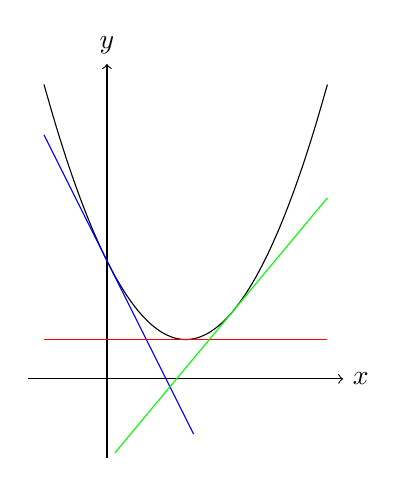
\begin{tikzpicture}
	      \draw[->] (-1,0) -- (3,0) node[right] {$x$};
	      \draw[->] (0,-1) -- (0,4) node[above] {$y$};
	      \draw[domain=-0.8:2.8,smooth,variable=\x,black] plot ({\x},{\x*\x-2*\x+1.5});
				\draw[domain=-0.8:1.1,smooth,variable=\x,blue] plot ({\x},{-2*\x+1.5});
				\draw[domain=-0.8:2.8,smooth,variable=\y,red] plot ({\y},{0.5});
				\draw[domain=0.1:2.8,smooth,variable=\x,green] plot ({\x},{1.2*\x-1.06});
	  \end{tikzpicture}
	\end{center}

	\subsection*{Delni odvodi}
	\paragraph{}
	Funkcija je odvisna od večih spremenljivk, zato jo moramo odvajati za vsako spremenljivko posebej. Ker nam odvod ene spremenljivke pove kako se funkcija obnaša samo po tej spremenljivki, temu rečemu delni odvod.


	$$\frac{\partial \varepsilon}{\partial a} =
		\sum_{i=1}^{N} 2 \frac{\partial (a x_i - b - y_i)}{\partial a} =
		2 \sum_{i=1}^{N} (a x_i - b - y_i)x_i$$

	$$\frac{\partial \varepsilon}{\partial b} =
		\sum_{i=1}^{N} 2 \frac{\partial (a x_i - b - y_i)}{\partial b} =
		2 \sum_{i=1}^{N} (a x_i - b - y_i)(-1) = -2 \sum_{i=1}^{N} (a x_i - b - y_i)$$

	Rešitev najdemo tako, da ugotovimo, pri katerih $a$ in $b$ sta odvoda enaka 0. To lahko rešimo z uporabmo matrik, vendar tega ne znamo, zato se bomo tega lotili s primitvno metodo gradientnega spusta.

	\section*{Gradientni spust}
	\paragraph{}
	Gradient nam pove smer največjega naraščanja funkcije. Gradient funkcije f(x) je vektor definiran kot:
	$$\nabla f = \begin{pmatrix}\frac{\partial f}{\partial x_{1}} & \frac{\partial f}{\partial x_{2}} & \frac{\partial f}{\partial x_{3}} & ... & \frac{\partial f}{\partial x_{n}}\end{pmatrix}$$

	V našem primeru linearne regresije je gradientni spust:
	$$\nabla \varepsilon =
	\begin{pmatrix}
	\frac{\partial \varepsilon}{\partial a} &
	\frac{\partial \varepsilon}{\partial b}
	\end{pmatrix}$$

	\paragraph{}
	Ker iščemo minimum funckije se bomo premikali v nasprotno smer gradienta. Spremembo spremenljivke $a$ lahko zapišemo kot:
	$$\Delta a = -(\nabla \varepsilon)_1 \cdot \lambda$$
	kjer $\lambda$ predstavlja velikost premika.

	Naše nove spremenljivke so:
	$$ a = a + \Delta a$$
	$$ b = b + \Delta b$$

	\paragraph{}
	S tem smo se premaknili za en korak bližje minimumu funkcije, to pomeni parametroma $a$ in $b$ pri katerih se bo premica najbolje prilegala na"sim to"ckam. Ta postopek ponovimo še n-krat. Večkrat ko ga ponovimo, bolj natančen bo naš rezultat.

	\paragraph{}
	Natančnost našega rezultata je odvisna tudi od $\lambda$ (velikost premika) in začetnih vrednost spremenljivk $a$ in $b$. Z manjšo velikostjo premika bo rezultat bolj natančen, vendar bomo morali postopek večkrat ponoviti. Ker s postopkom isčemo samo lokalne minimume, nam začetna vrednost spremenljivk določi kateri minimum bomo našli.


	\section*{Linerana regresija elipse}
	\paragraph{}
	Imamo $N$ točk krožnice nekega planeta $T_1(x_1, y_1), T_2(x_2, y_2) \ldots, T_n(x_n, y_n)$. Podobno kot pri prej"snjem primeru, bomo tudi tokrat iskali funkcijo, ki se to"ckam najbolj prilega. Tokrat bomo namesto premice iskali elipso, saj se elipsa seveda bolj prilega kro"znici planeta kot pa premica.


	Elipsa je sto"znica, zato zapišemo splošno enačbo za sto"znice:
	$$Ax^2 + Bxy + Cy^2 + Dx + Ey + F = 0$$

	\paragraph{}
	Tako kot prej se nam bo pojavila napaka, ki jo ozna"cimo z $\varepsilon$.
	$$\varepsilon_i = Ax_i^2 + Bx_iy_i + Cy_i^2 + Dx_i + Ey_i + F$$
	Za razliko od premice, je oblika sto"znice odvisna od "sestih parametrov namesto dveh. To so: $A, B, C, D, E$ in $F$. Zato bomo torej spreminjali teh "sest parametrov.

	\paragraph{}
	Podobno kot pri premici najprej definiramo skupno napako kot vsoto kvadratov vseh napak:
	\[\varepsilon = \sum_{i=1}^{N}\varepsilon_i\]
	\[\varepsilon = \sum_{i=1}^{N} (Ax_i^2 + Bx_iy_i + Cy_i^2 + Dx_i + Ey_i + F)^2\]

	\paragraph{}
	Enako kot pri premici moramo na"so napako delno odvajati po spremenjivkah od katerih je na"sa napaka odvisna, da bomo znali te spremenljivke spreminjati pravilno. To pomeni da potrebujemo izra"cunati delni odvod napake po $A, B, C, D, E$ in $F$. Delni odvodi za ena"cbo sto"znic so:

	$$\frac{\partial \varepsilon}{\partial A} = \sum_{i=1}^{N}2(Ax_i^2 + Bx_iy_i + Cy_i^2 + Dx_i + Ey_i + F)(x_i^2)$$
	$$\frac{\partial \varepsilon}{\partial B} = \sum_{i=1}^{N}2(Ax_i^2 + Bx_iy_i + Cy_i^2 + Dx_i + Ey_i + F)(x_iy_i)$$
	$$\frac{\partial \varepsilon}{\partial C} = \sum_{i=1}^{N}2(Ax_i^2 + Bx_iy_i + Cy_i^2 + Dx_i + Ey_i + F)(y_i^2)$$
	$$\frac{\partial \varepsilon}{\partial D} = \sum_{i=1}^{N}2(Ax_i^2 + Bx_iy_i + Cy_i^2 + Dx_i + Ey_i + F)(x_i)$$
	$$\frac{\partial \varepsilon}{\partial E} = \sum_{i=1}^{N}2(Ax_i^2 + Bx_iy_i + Cy_i^2 + Dx_i + Ey_i + F)(y_i)$$
	$$\frac{\partial \varepsilon}{\partial F} = \sum_{i=1}^{N}2(Ax_i^2 + Bx_iy_i + Cy_i^2 + Dx_i + Ey_i + F)$$

	\paragraph{}
	Da najdemo najbolj"se parametre, pri katerih bo funkcija imela najmanj"so napako, bomo ponovno uporabili gradientni spust. Za razliko od gradientnega spusti pri eni premici, bomo tokrat spreminjali "sest parametrov. Na"s gradient je torej:

	$$\nabla \varepsilon = \begin{pmatrix}
	\frac{\partial \varepsilon}{\partial A} &
	\frac{\partial \varepsilon}{\partial B} &
	\frac{\partial \varepsilon}{\partial C} &
	\frac{\partial \varepsilon}{\partial D} &
	\frac{\partial \varepsilon}{\partial E} &
	\frac{\partial \varepsilon}{\partial F}
 	\end{pmatrix}$$

	To pomeni da so na"se spremembe parametrov:

	$$\Delta A = -(\nabla \varepsilon)_1 \cdot \lambda$$
	$$\Delta B = -(\nabla \varepsilon)_2 \cdot \lambda$$
	$$\Delta C = -(\nabla \varepsilon)_3 \cdot \lambda$$
	$$\Delta D = -(\nabla \varepsilon)_4 \cdot \lambda$$
	$$\Delta E = -(\nabla \varepsilon)_5 \cdot \lambda$$
	$$\Delta F = -(\nabla \varepsilon)_6 \cdot \lambda$$

	Iz "cesar sledi, da so na"si novi parametri podobno kot pri premici:

	$$A = A + \Delta A$$
	$$B = B + \Delta B$$
	$$C = C + \Delta C$$
	$$D = D + \Delta D$$
	$$E = E + \Delta E$$
	$$F = F + \Delta F$$

	\paragraph{}Pravilnost na"sega rezultata je seveda odvisna od tega koliko ponovitev bomo naredili, kolik"sna bo na"sa $\lambda$ in kak"sne za"cetne vrednosti $A, B, C, D, E$ in $F$ smo si izbrali.

    \section*{Logistična regresija}
    \paragraph{}
    Glavna razlika med logistično in linearno regesijo je, da pri linearni regresiji določamo zvezno spremenljivko ($y$ je odvisen od $x$), medtem ko nam pri logistični regresiji model vrne kakšna je verjetnost, da vhodni podatki sodijo v določeno kategorijo.
    Zato se logistična regresija uporablja za klasifikacijo (npr. prepoznavanje števk idr.).


    \section*{Dodatno}
    \subsection*{Ekliptični koordinatni sistem}
    \paragraph{}
    Eden izmed koordinatnih sistemov za določanje lege nebesnih teles. Lokacijo določimo s tremi podatki. Ker so koordinate definirane glede na ravnino zemljine orbite, je $z$ koordinata za Zemljo vedno enaka 0.
    \begin{description}
        \item[$l$] longtituda, ekliptična dolžina, od $0^\circ$ do $360^\circ$.
        \item[$b$] latituda, ekliptična širina od $-90^\circ$ do $90^\circ$.
        \item[$r$] razdalja
    \end{description}

    \paragraph{}
    V kartezične koordinate podatke pretvorimo po formulah:
    $$x = r \cos b \cos l$$
    $$y = r \cos b \sin l$$
    $$z = r \sin b$$

    \paragraph{}
    Ker tiri vseh planetov ležijo v (skoraj) isti ravnini, bomo $z$ koordianto zanemarili.


\end{document}
